%% demo.tex
%%
%% Time-stamp: <2009-12-05 emarsden>


\section{Démonstration}

\frame[plain]{  \heading{Plan de la Présentation}
\ecmsetupplan
\begin{itemize}
  \item[\small $\Diamond$] Introduction
  \item[\small $\Diamond$] Fonctionnement
  \item[\small $\Diamond$] {\color{purple}\textbf{Démonstration}}
  \item[\small $\Diamond$] Applications
  \item[\small $\Diamond$] Conclusions
\end{itemize}
}


\frame{ \heading{Démo: créer une carte personnalisée}  \vfill
  \begin{minipage}{0.45\textwidth}
    \begin{enumerate}
    \item Trouver la zone pertinente dans le slippymap
    \item Ouvrir le tab ``Export''
    \item Sélectionner le format (PDF, SVG, PNG, XML)
    \item Exporter
    \item Éditer le SVG dans Inkscape
    \end{enumerate}
  \end{minipage} \quad %
  \begin{minipage}{0.49\textwidth}
    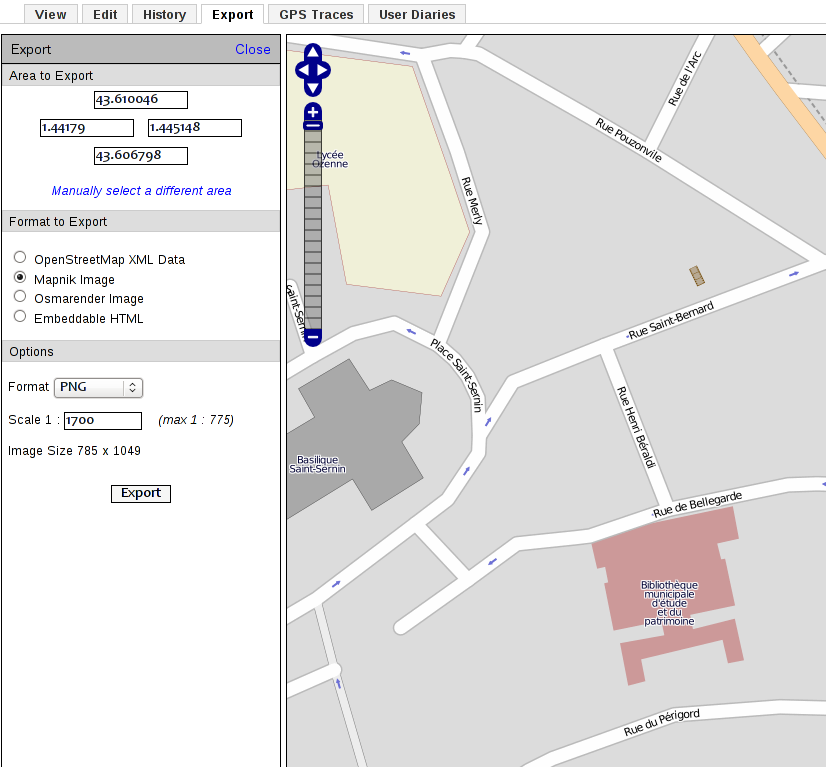
\includegraphics[width=\textwidth]{figures/OSM-export}
  \end{minipage}
}



\frame{ \heading{Démo: corriger un nom de rue}  \vfill
  \begin{minipage}{0.45\textwidth}
    \begin{enumerate}
    \item Trouver la rue dans le slippymap
    \item Ouvrir le tab ``Edit''
    \item S'identifier
    \item Sélectionner la voie
    \item Changer le nom
    \end{enumerate}
  \end{minipage} \quad %
  \begin{minipage}{0.49\textwidth}
    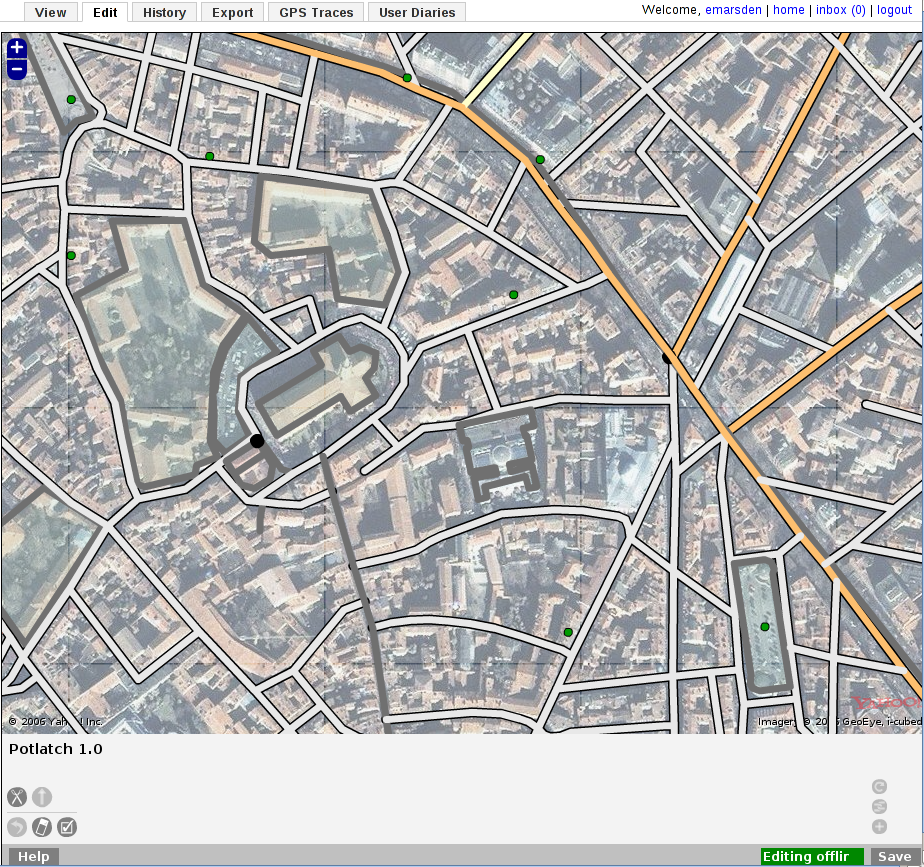
\includegraphics[width=\textwidth]{figures/potlatch}
  \end{minipage}
}


\frame{ \heading{Démo: ajouter une voie cyclable}  \vfill
  \begin{minipage}{0.45\textwidth}
    \begin{enumerate}
    \item Ouvrir JOSM
    \item Télécharger la zone pertinente
    \item Sélectionner la voie
    \item Découper le tronçon pertinent
    \item Ajouter tag \texttt{cycleway=left}
    \end{enumerate}
    \end{minipage} \quad %
  \begin{minipage}{0.49\textwidth}
    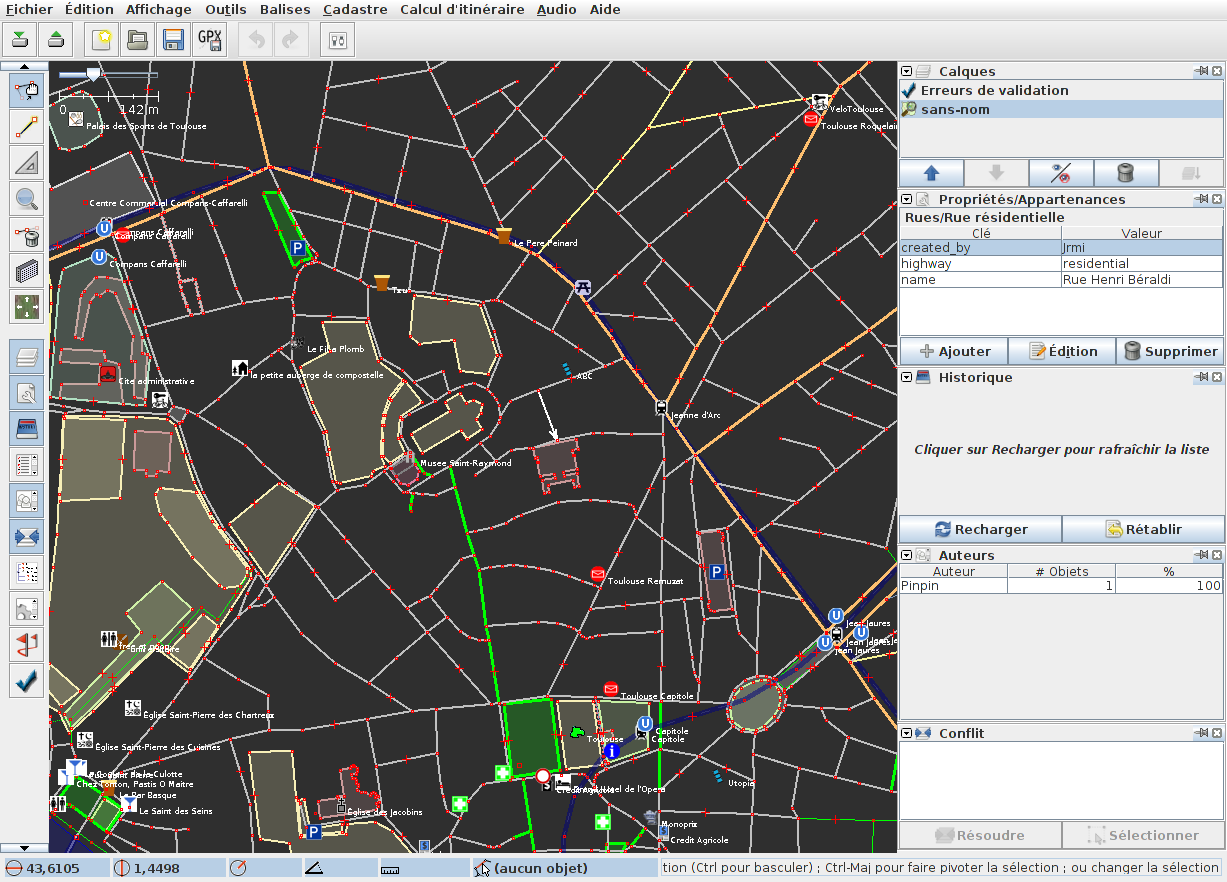
\includegraphics[width=\textwidth]{figures/JOSM}
  \end{minipage}
}

\frame{ \heading{Démo: ajouter son bar favori}  \vfill
\begin{enumerate}
\item Ouvrir JOSM et télécharger la zone pertinente
\item Récupérer une vue cadastre de la zone (ou waypoint GPS)
\item Créer un n\oe{}ud au bon endroit
\item Ajouter des tags \texttt{amenity=bar} (ou \texttt{pub} ou \texttt{nightclub})
\item Préciser le nom du bar en ajoutant un tag \texttt{name=La Tireuse}
\item Uploader les données
\end{enumerate}
}

\frame{ \heading{Démo: tracer une nouvelle route depuis un gpx}  \vfill
\begin{enumerate}
\item Néttoyer le fichier gpx de points inutiles
\item Ouvrir le tab ``GPS Traces''
\item S'identifier
\item Uploader son fichier gpx
\item Télécharger la zone dans JOSM
\item Tracer depuis la couche gpx
\end{enumerate}
}

\frame{ \heading{Démo: Lakewalker pour tracer un lake}  \vfill
\begin{enumerate}
\item Installer les plugins lakewalker \& WMS
\item Naviguer vers une zone avec un lac
\item Récupérer un fond Landsat pour la zone
\item Activer le plugin lakewalker
\item Vérifier les données
\item Uploader les changements
\end{enumerate}
}



%% new typographic/map explosion
%% http://calebwaldorf.net/reblog/typologies-from-the-new-cartographic-explosion/



%% EOF
